%%%%%%%%%%%%%%%%%%%%%%%%%%%%%%%%%%%%%%%%%
% University Assignment Title Page
% LaTeX Template
% Version 1.0 (27/12/12)
%
% This template has been downloaded from:
% http://www.LaTeXTemplates.com
%
% Original author:
% WikiBooks (http://en.wikibooks.org/wiki/LaTeX/Title_Creation)
%
% License:
% CC BY-NC-SA 3.0 (http://creativecommons.org/licenses/by-nc-sa/3.0/)
%
% Instructions for using this template:
% This title page is capable of being compiled as is. This is not useful for
% including it in another document. To do this, you have two options:
%
% 1) Copy/paste everything between \begin{document} and \end{document}
% starting at \begin{titlepage} and paste this into another LaTeX file where you
% want your title page.
% OR
% 2) Remove everything outside the \begin{titlepage} and \end{titlepage} and
% move this file to the same directory as the LaTeX file you wish to add it to.
% Then add \input{./title_page_1.tex} to your LaTeX file where you want your
% title page.
%
%%%%%%%%%%%%%%%%%%%%%%%%%%%%%%%%%%%%%%%%%

%----------------------------------------------------------------------------------------
%	PACKAGES AND OTHER DOCUMENT CONFIGURATIONS
%----------------------------------------------------------------------------------------

\documentclass[12pt]{article}
\usepackage{graphicx}
\usepackage{caption}
\usepackage{subcaption}
\usepackage{listings}
\usepackage{xcolor}
\usepackage{mathtools}
\begin{document}
\begin{titlepage}

\newcommand{\HRule}{\rule{\linewidth}{0.5mm}} % Defines a new command for the horizontal lines, change thickness here

\center % Center everything on the page

%----------------------------------------------------------------------------------------
%	HEADING SECTIONS
%----------------------------------------------------------------------------------------

\textsc{\LARGE McGill University}\\[1.5cm] % Name of your university/college
\textsc{\Large COMP 521}\\[0.5cm] % Major heading such as course name
\textsc{\large Modern Computer Games}\\[0.5cm] % Minor heading such as course title

%----------------------------------------------------------------------------------------
%	TITLE SECTION
%----------------------------------------------------------------------------------------

\HRule \\[0.4cm]
{ \huge \bfseries TerraGen: Procedural Terrain Generation and Resource Analysis}\\[0.4cm] % Title of your document
\HRule \\[1.0cm]

%----------------------------------------------------------------------------------------
%	AUTHOR SECTION
%----------------------------------------------------------------------------------------

\begin{minipage}{0.4\textwidth}
\begin{flushleft} \large
Benjamin \textsc{San Souci} \\ % Your name
Maude \textsc{Lemaire} % Your name
\end{flushleft}
\end{minipage}
~
\begin{minipage}{0.4\textwidth}
\end{minipage}\\[4cm]

% If you don't want a supervisor, uncomment the two lines below and remove the section above
%\Large \emph{Author:}\\
%John \textsc{Smith}\\[3cm] % Your name

%----------------------------------------------------------------------------------------
%	DATE SECTION
%----------------------------------------------------------------------------------------

{\large \today}\\[3cm] % Date, change the \today to a set date if you want to be precise

%----------------------------------------------------------------------------------------
%	LOGO SECTION
%----------------------------------------------------------------------------------------

%\includegraphics{Logo}\\[1cm] % Include a department/university logo - this will require the graphicx package

%----------------------------------------------------------------------------------------

\vfill % Fill the rest of the page with whitespace

\end{titlepage}

\section{Introduction}

TerraGen aims to generate realistic island terrains using a relaxed polygonal map and assigning biomes based on simulated moisture and elevation. Following the map generation process, the city generation algorithm analyzes the terrain and produces a  set of cities with unique statistics directly related to their location and access to resources.

Island generation was modeled after Amit Patel's ``Polygonal Map Generation for Games''\cite{Patel:2010:Online}, where Chrisophe Le Besnerais's JavaScript version, ``Island.js''\cite{LeBesnec:2015:Online} was extended to accommodate for additional features. First a graph structure of polygons is generated, then annotated with elevation, moisture, and labeled as either land or water. In order to generate a more natural-looking island, Voronoi polygons were generated and relaxed using an implementation by Raymond Hill \cite{Hill:2015:Online}. Extensions to the implementation included adding fishing regions, minerals, volcanoes, tectonic plates, forest density, and fauna abundance.

The TerraGen city statistic generation addresses a problem that has been little discussed in the scope of games beyond the intersection of geography information systems (GIS) and 3D game engines. Using the generated plot, the city generation algorithm finds a suitable location at which to place a city. From this location, resources in close proximity are identified and used in determining the city's population size, army size, happiness level and wealth, among other features.

The result is a randomly generated island with over two dozen biomes, oceanic regions, dispered minerals and a handful of cities. A sample map at different stages of generation is included in the methodology portion of the report.

The project was separated into two major components: the terrain generation and extensions, and the city statistics generation. Maude was mainly responsible for the terrain generation portion of the project and the majority of the final report. Benjamin produced the city generation algorithm. Both team members collaborated on the methods by which terrain analysis and terrain generation were extended.

\section{Background}
Map generation has been a important focus within the gaming industry in recent years as a means of promoting re-playability without having to manually generate a large number of maps. By randomly generating a map with new instances of a game, the players must face new challenges and adapt their game-play to suit the new terrain. A wide range of approaches already exist, with varying levels of complexity and randomness.

\subsection{Grids}
Terrains are typically built off of a grid system; this can be a simple tile-based square grid, a hexagonal grid, or a polygonal grid either composed of randomly sized convex shapes or relaxed polygons. Figure 1 displays the difference between each of these grid types and how ``natural'' each of these appear in island generation.

\begin{figure}
        \centering
        \begin{subfigure}[b]{0.45\textwidth}
                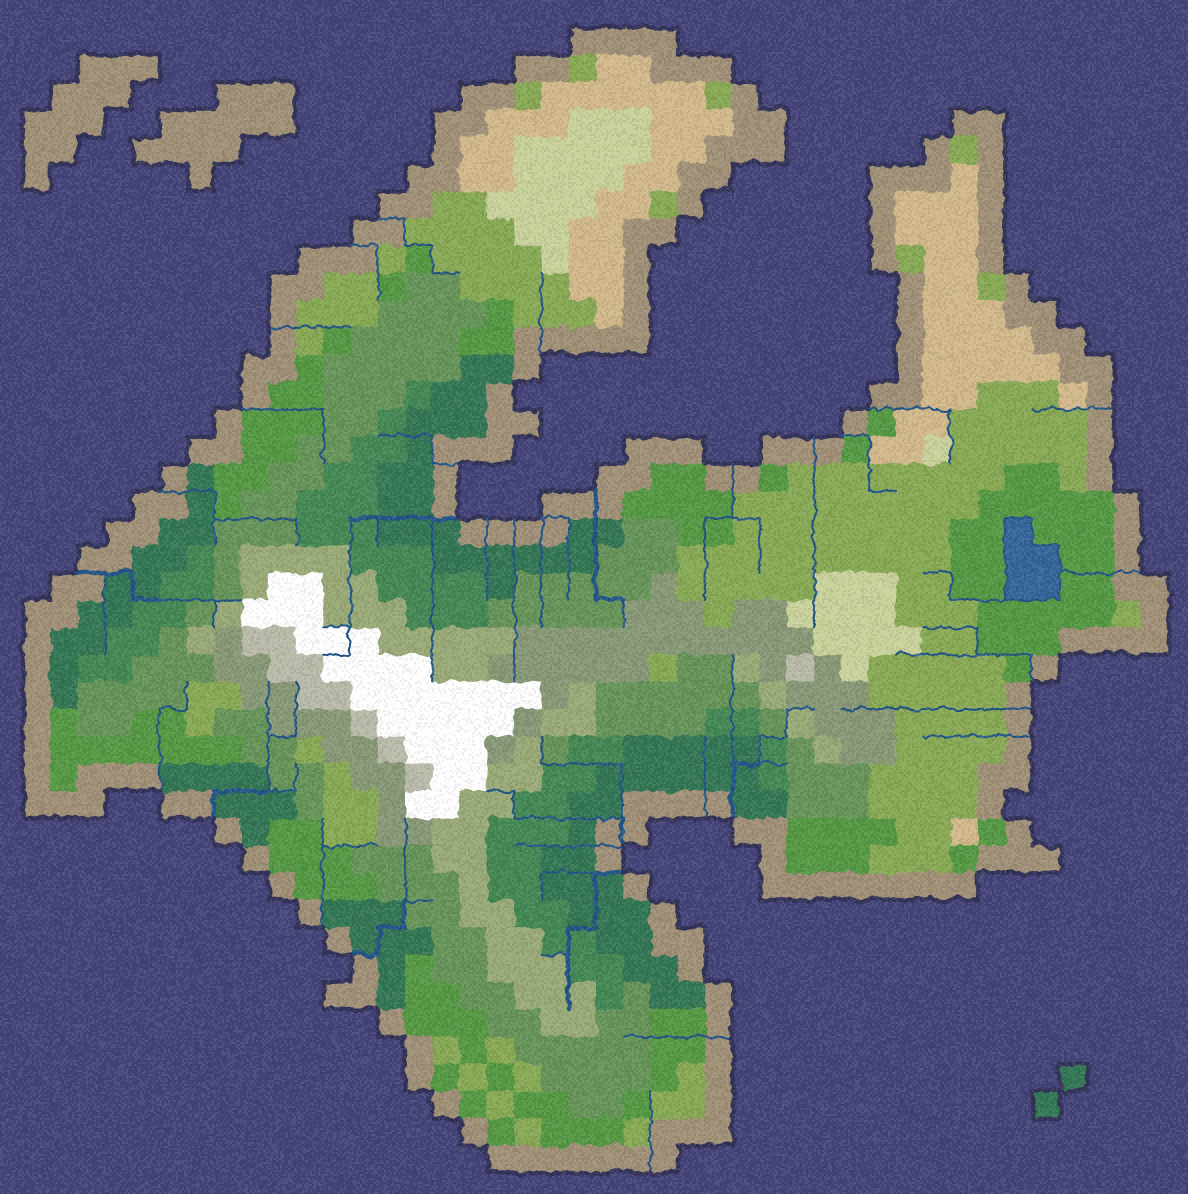
\includegraphics[width=\textwidth]{Square.png}
                \caption{Square Grid}
                \label{fig:Square}
        \end{subfigure}%
        ~ %add desired spacing between images, e. g. ~, \quad, \qquad, \hfill etc.
          %(or a blank line to force the subfigure onto a new line)
        \begin{subfigure}[b]{0.45\textwidth}
                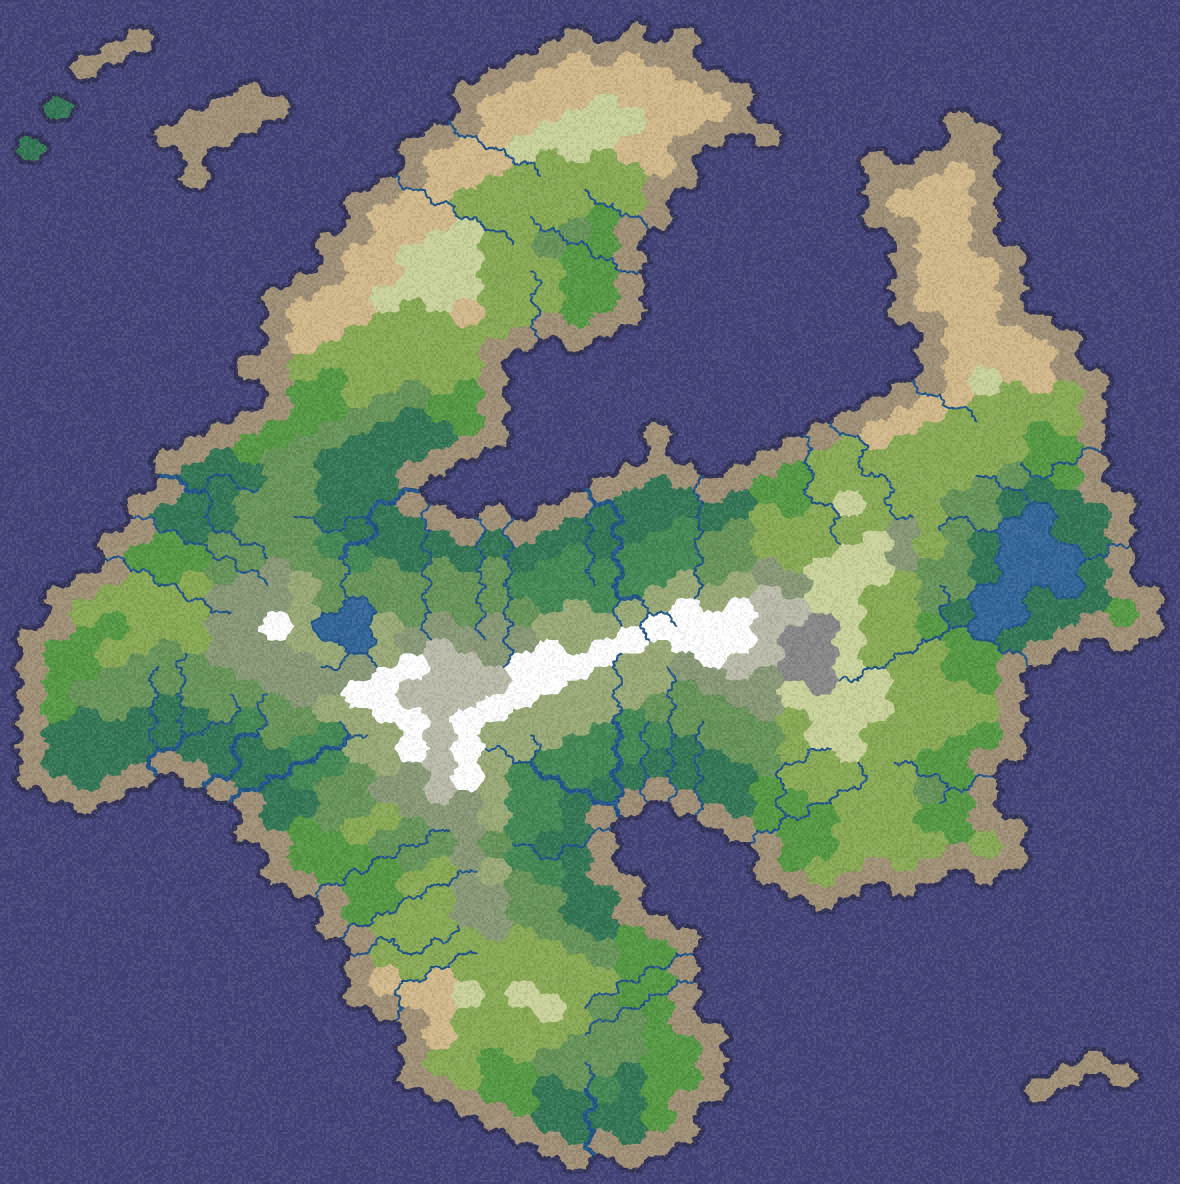
\includegraphics[width=\textwidth]{Hex.png}
                \caption{Hexagonal Grid}
                \label{fig:Hex}
        \end{subfigure}
        ~ %add desired spacing between images, e. g. ~, \quad, \qquad, \hfill etc.
          %(or a blank line to force the subfigure onto a new line)
        \begin{subfigure}[b]{0.45\textwidth}
                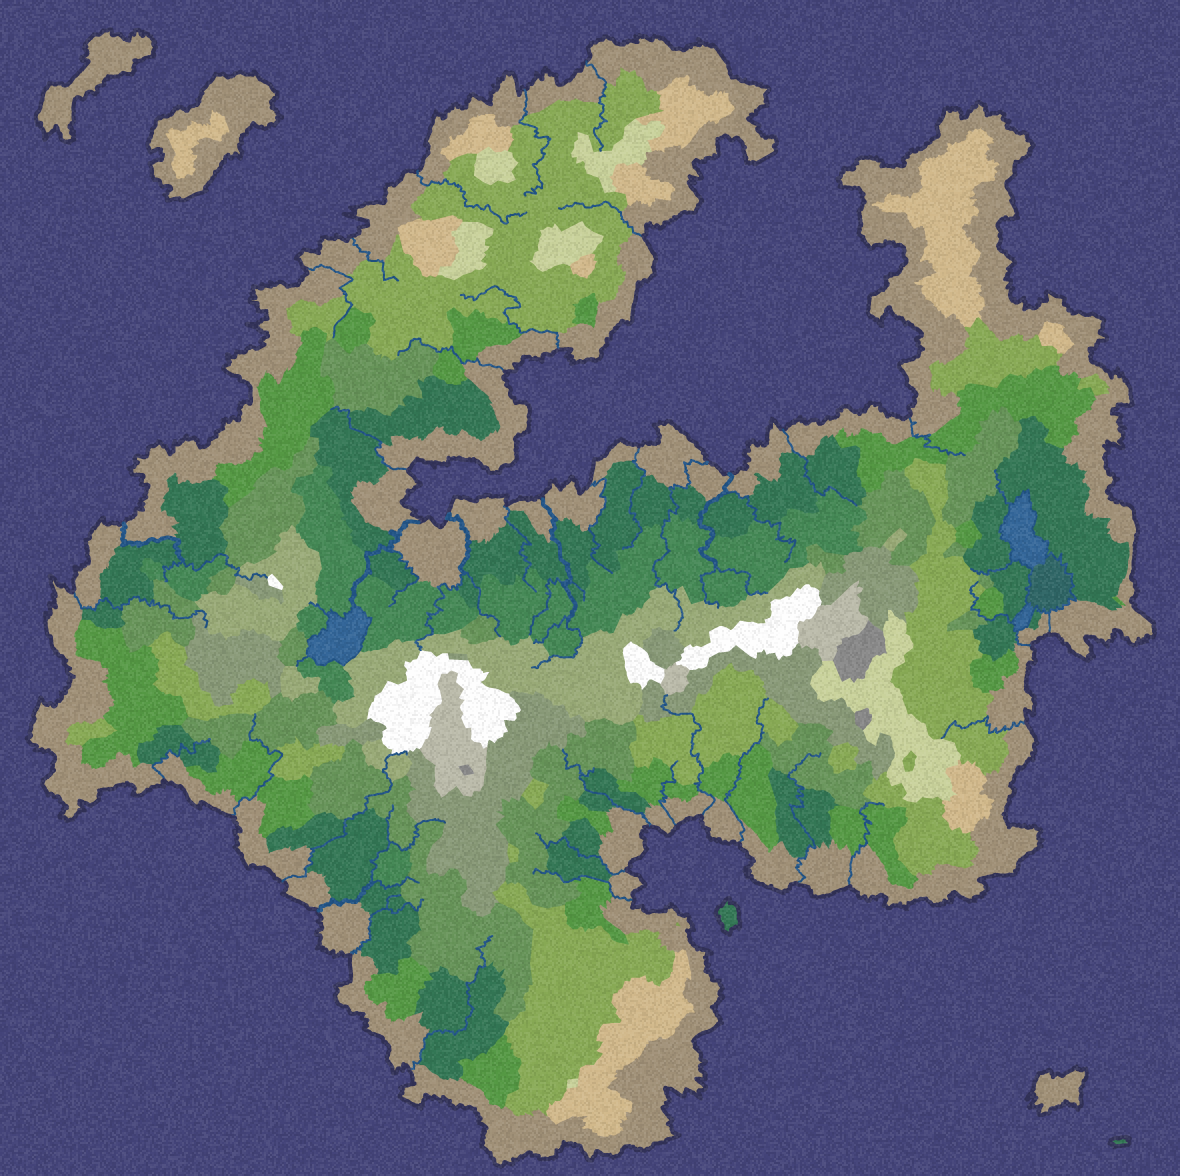
\includegraphics[width=\textwidth]{Random.png}
                \caption{Random Polygon Grid}
                \label{fig:Random}
        \end{subfigure}
        \begin{subfigure}[b]{0.45\textwidth}
                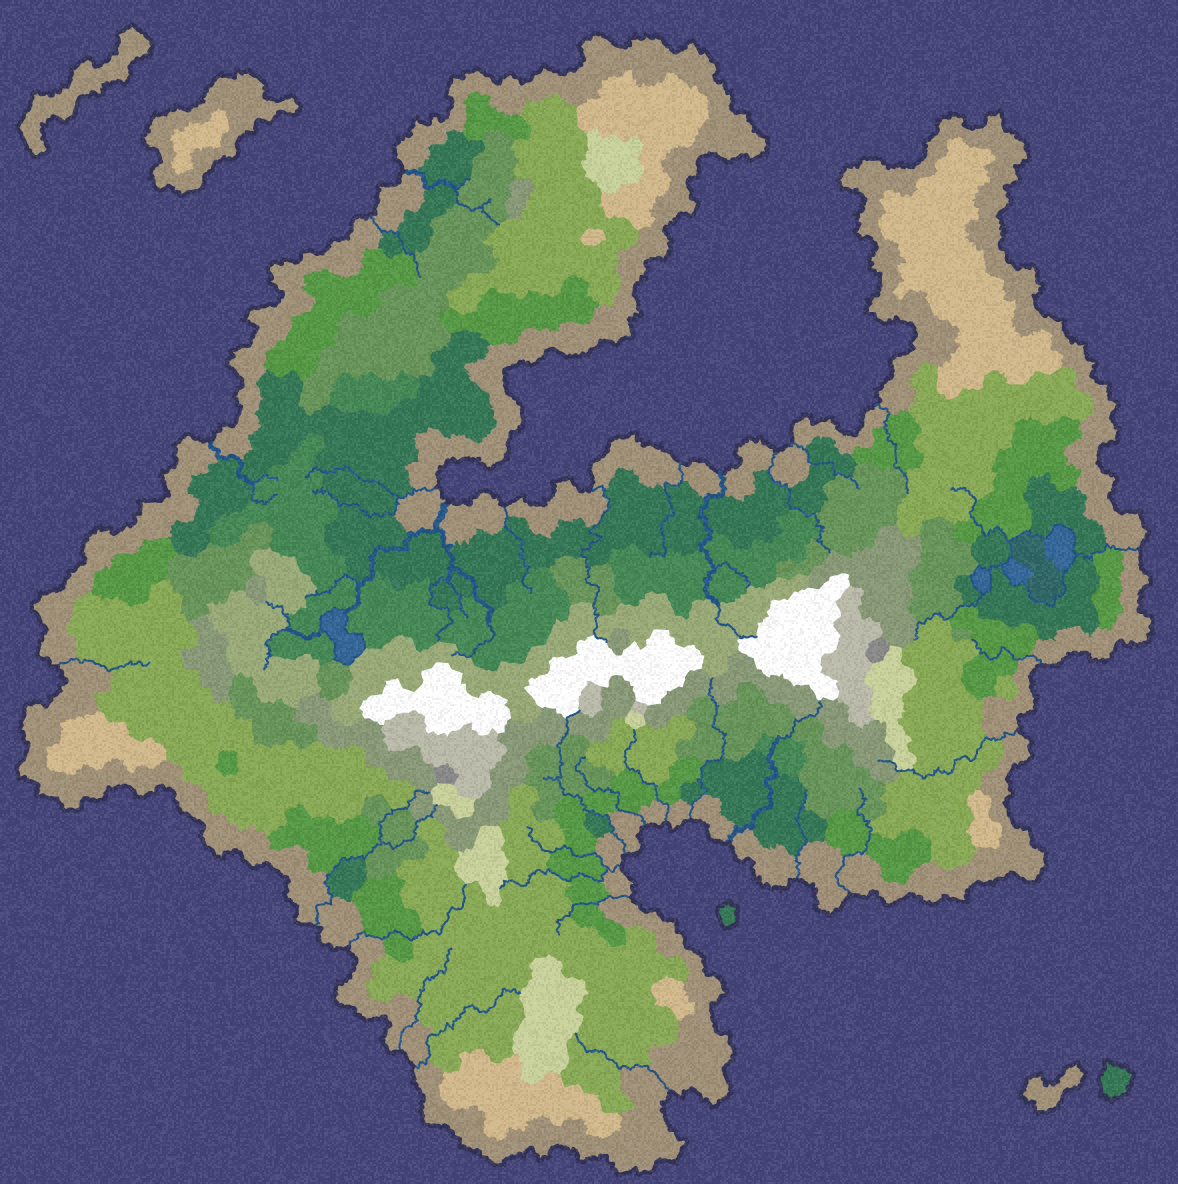
\includegraphics[width=\textwidth]{Relaxed.png}
                \caption{Relaxed Polygon Grid}
                \label{fig:Relaxed}
        \end{subfigure}
        \caption{Islands generated using Amit Patel's demo. Each is generated using Perlin noise, displays biomes, and demonstrates the use of different grid types.}\label{fig:gridtypes}
\end{figure}

Hexagonal grids and polygonal grids typically provide the most natural-looking islands. Hexagonal grids have been extensively developed by academics such as Clark Verbrugge\cite{Verbrugge:1997:Online}, and can be perturbed to add irregularity. Polygonal grid generation has mainly revolved around randomly generating a series of Voronoi polygons. A number of algorithms generate Voronoi diagrams based on a set of random points (Fortune's algorithm\cite{Fortune:1986:SAV:10515.10549}), a set area (Lloyd's algorithm\cite{doi:10.1137/S0036144599352836}) or Delaunay triangulations (Bowyer-Watson algorithm\cite{Watson01011981}). In particular, the set of points upon which the polygons are generated can be mapped to known natural phenomena. For example, researchers at the Universit\'{e} de Lyon,generated Voronoi diagrams based on hydrology \cite{Genevaux:2013:TGU:2461912.2461996}. As an extension, Lloyd relaxation can be used to distribute points more evenly for diagram generation.

Following Patel's polygonal map generation methods, once a Voronoi diagram is generated, the internal representation consists of nodes and edges; the first is used for identifying adjacent polygons. The second represents the Delaunay triangulation which can be used for pathfinding. Conceptually, every corner in the triangulation corresponds to a polygon center and every edge to an edge in the diagram. As polygons in the map are irregular, it is difficult to make assumptions about neighboring cells and paths from one point to another; this representation ensures that the map is traversed in a meaningful way throughout the generation process.

\subsection{Islands}

Realistic islands must maintain a rather circular shape, with some random variation. A radial function is suggested, using sine waves to produce a round island. The island is generated according to polar coordinates stemming from the center of the canvas. Depending on the sine waves, the island can resemble an octopus, with thin strips of land extended from the center of the island.

Alternatively, Perlin noise can be generated and used to control the shape of the island given some constraints. This method provides more realistic island shapes due to the fact that Perlin noise consists of visual details of equal size; this gives a more controlled random appearance, closely imitating natural textures.

Once land polygons have been identified, ocean is filled in from the edges and any remaining ``water'' polygons unreachable from the fringe of the map (landlocked) are marked as lakes.

\subsubsection{Elevation}
In generating terrains, in order to provide a more realistic map, a natural-looking elevation must be assigned to each grid unit. Some typical approaches include using Perlin noise, fractal landscapes, or real-world data. Simpler and less computation-intensive attempts at generating elevation focus on assigning a maximum elevation to a central point on the island and gradually decreasing the elevation according to a cumulative distribution until the lowest elevation point (the ocean) has been reached\cite{Patel:2010:Online}.

Perlin noise is a popular technique due to the fact that it successfully generates  realistic textures (as previously discussed under island generation). One of the drawbacks of using Perlin noise in elevation generation is that there tends to be a rather uniform distribution to the terrain height and few realistic peaks and valleys typical of natural landscapes. A number of approaches go beyond using strict Perlin noise generation and instead focus on value noise, a less mathematically-involved method which may be calibrated to take actual geographical data into account \cite{Parberry:2014}.

Fractal landscapes can provide a pseudo-random terrain elevation; these landscapes focus on self-similarity, where subsets of the object resemble (or are identical to) the whole. Recursive algorithms such as the diamond-square algorithm use midpoint-displacement in order to generate heightmaps. The resulting meshes can be masked over a terrain to provide elevation information \cite{Martz:1997:Online}.

Each of these methods can be further improved by simulating natural phenomena such as erosion and plate tectonics. In particular, terrain (and specifically elevation) can be simulated entirely according to plate tectonics; although computation-heavy, this approach results in the most realistic elevation map, and can be used to add features such as earthquake risk zones and volcanoes \cite{Key}.

Whatever approach is used, the resulting elevation map must be applied to the map grid; this can be done by assigning an elevation to each corner, or center of a grid unit. Given a polygonal map (or hexagonal map with more than four corners per grid unit), assigning elevations to corners yields a more complex elevation model with a greater number of discrete steps. Greater detail is key as elevation is then used to derive biomes and rivers later in the terrain generation process.

\subsubsection{Rivers and Moisture}
Based on the previously determined elevation model, rivers can be traced from a point of high elevation to the ocean. As rivers tend to be thinner than a single grid unit, a more realistic visualization approach involves tracing rivers alongside the edges of grid units, whether they be tiles, hexagons or polygons.

Water-flow models can be further developed by taking into consideration the amount of moisture available at a given starting point. For instance, it is more probable for a river to stem from a snowy mountaintop than a tundra or bare terrain. Instead of drawing strictly uniform-width rivers, rivers can be widened according to surrounding elevation and water availability from a given source; tributaries can combine to form a larger river emptying into the ocean \cite{Genevaux:2013:TGU:2461912.2461996}.

Depending on the order of the approach taken (rivers generated first or moisture generated first), areas of high moisture could be assigned to those in closer proximity to lakes and rivers, or more lakes and rivers could form in areas of higher moisture. Typically, moisture is mapped to distance from the ocean and elevation. In either means of terrain generation, moisture is modeled after known hydrology models such as those discussed by G\'enevaux and his team \cite{Genevaux:2013:TGU:2461912.2461996}.

In summary, moist, fertile soil occurs in areas near rivers and lakes. This soil leads to thicker vegetation growth, which in turn slows water flow. Rainfall may vary according to area, but flows downhill in all instances, gaining momentum and pooling in springs, rivers and lakes as it travels towards the ocean.

\subsubsection{Biomes and Minerals}

Biomes are generated according to moisture and elevation. Depending on the range of values given to each of these features, a wide range of biomes can be simulated. Assuming the elevation and moisture maps demonstrate gradual changes Due to gradual change in moisture and elevation, biomes will be assigned to groups of grid units and rarely result in isolated single-unit regions. Patel proposes a model consisting of fifteen biomes as shown in Figure 2.

\begin{figure}
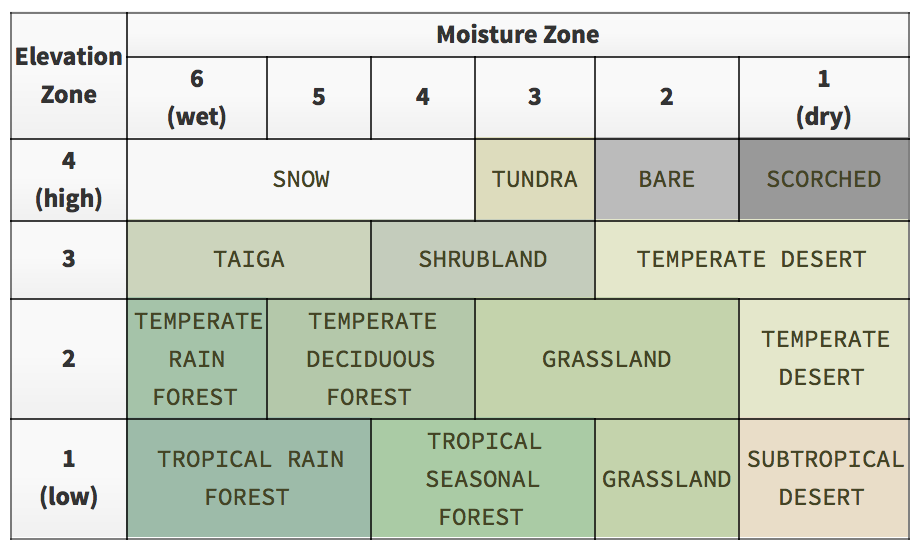
\includegraphics[width=\textwidth]{Biomes.png}
\caption{Biomes According to Elevation and Moisture}
\end{figure}

Each biome can be associated with a set of flora of fauna, distinct to its features. For example, although tropical rain forests cover only 7\% of the earth's surface area, they are home to over 50\% of the earth's species. A multi-layered forest directly contributes to the spread of nutrients and perpetuation of the nitrogen, oxygen and carbon cycles \cite{Robinson:2008:Online}.

With every terrain comes resource distribution, including important minerals. Minerals form according to the heating and cooling of molten materials, pressure within the ground, and evaporation of liquids \cite{9780939950812}. As such, minerals form within set biomes with different levels of rarity depending on the precise conditions under which they are produced. For instance, gold is mainly found near the earth's core, although veins of gold are gradually being exposed to the surface and eroding away. Due to its weight, gold can become concentrated in hollows and trapped in beds of rivers. A range of mines and corresponding minerals across the globe can be seen in Figure 3.

\begin{figure}
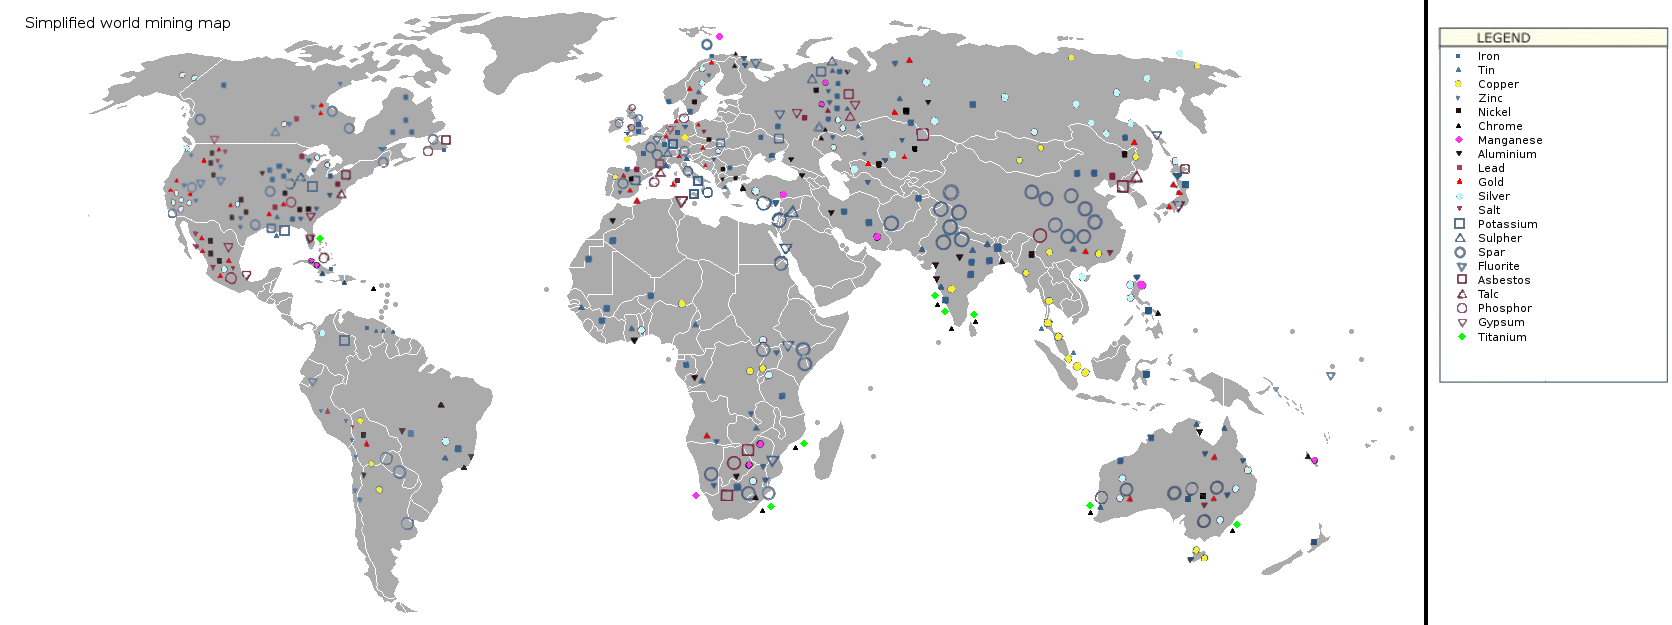
\includegraphics[width=\textwidth]{mining.png}
\caption{Mines across the world}
\end{figure}

\subsection{Terrain Analysis}
Terrain analysis has been little studied beyond urban development in the scope of video games. In recent years, there has been a push towards combining geography information systems (GIS) and gaming. GIS are mainly used for scientific research purposes in the area of geoinformatics; the systems are aimed at designed to capture, store, manipulate, analyze, and present spatial and geographical data. By combining these analytical features with gaming, the industry can produce more realistic scenarios. Understanding how players can interact with geographical features and resources found on the terrain could be a natural extension of including GIS in gaming \cite{Borneman:2011:Online}.

Procedural city growth and urban development within the gaming world has mainly revolved around urban, modern settings dealing with multi-story buildings and complex grids of roads and highways. In fact, companies have focused efforts towards building software capable of generating cities. Electronic Arts has released a tool known as CityEngine, specifically used for city generation in their Need for Speed game series\cite{10.1109/MCG.2008.58}. In regards to medieval cities and little-developed civilizations, although many games revolve around this theme, there has been fewer attempts at procedurally generating such environments.

\section{Methodology}

TerraGen was built as an extension to an existing JavaScript implementation of Patel's polygonal map generation method, written by Christophe Le Besnerais \cite{LeBesnec:2015:Online}. This implementation provided a relaxed polygonal grid, with basic elevation and moisture mapping, and a simple waterflow model. The terrain analysis portion of the implementation was generated from scratch, and driven by the provided island map.

Le Besnerais's implementation uses client-side JavaScript to render a map on an HTML5 canvas using Paper.js\cite{Lehni:2015:Online}, a JavaScript implementation of Voronoi diagrams by Raymond Hill \cite{Hill:2015:Online} and a Perlin noise generator by Sean McCullough\cite{McCullough:2015:Online}. Built-in functionality included basic island generation and biome assignment.

\subsection{Island Generation}
As provided with the existing implementation, terrains are generated on top of a relaxed polygonal grid. Island shape and size is determined by a randomly generated Perlin noise patch of given height and width (which can be seen as a separate \texttt{canvas} item within the rendered web page). Islands are highly configurable; a list of customizable parameters are shown in Listing 1. For the remainder of the report, it will be assumed that the island generated has a Perlin width and height of 350, canvas width and height of 1,000 and 50,000 polygons.

\begin{lstlisting}[caption=Island Parameters]
Island.init({
	width: 1000,
	height: 1000,
    perlinWidth: 350,
    perlinHeight: 350,
    allowDebug: false,
    nbSites:50000,
    maxRiversSize: 1000,
    shading:0,
    nbGraphRelaxation: 0,
    shadeOcean:false
});
\end{lstlisting}

\subsection{Elevation}
A simple elevation mapping was included in the base Island.js code. In this implementation, elevation is set at each corner of every polygon as the distance from the coast where water polygons do not contribute to the distance. A secondary pass is performed to redistribute the elevations to match the following cumulative distribution: $$y(x) = 1 - (1-x)^2$$.

This further ensures that elevation the ocean will always be reached when traveling downhill.

The provided elevation was extended to accomodate for
Additional features such as plate tectonics and volcanoes were simulated on top of the generated elevation.

Used to map to fishing areas and randomized throughout the ocean.

\subsection{Rivers}
Allowed to pool into lakes and lake were allowed to empty into the ocean. Lake colors are distributed according to depth.

\subsection{Biomes}
Ice was added as an additional biome

\subsection{Minerals}
Unique extension beyond the basic features provided in the starter code.

\subsection{Terrain Analysis}
The intent behind TerraGen's terrain analysis is to generate initial statistics for cities. After the island is generated, the terrain analysis portion of the implementation receives the grid. Six cities are randomly distributed on the island, with randomly assigned curiosity and aggressiveness attributes. Listing 2 demonstrates a sample city JSON item.

\begin{lstlisting}[caption=JSON City Item]
{
  center: center1,
  resources: {
    vegetables: 0,
    meat: 0,
    wood: 0,
    minerals: {
      copper: 0,
      iron: 0,
      gold: 0,
      titanium: 0,
      silver: 0,
      coal: 0,
      gems: 0,
      aluminium: 0,
      lead: 0,
      nickel:0,
      uranium:0,
      zinc:0
    }
  },
  populationSize: 100,
  armySize: 0,
  location: [center1],
  curiosity: 1.5,
  aggressiveness: 0.2,
  technology: 0,
  artistNumber: 0,
  economy: 0
};
\end{lstlisting}

The above statistics and features are calculated using a simple update loop, which consists of the following steps:

\begin{enumerate}
\item Randomly generate city aggressiveness (value between 0 and 0.5) and city curiosity (value between 0 and 2).
\item Expand the territory of the city.
\item Increase city resources based on controlled territory.
\item Increase population.
\item Calculate economical power of city.
\item Calculate number of artists within the city.
\item Calculate technological advancement.
\item Calculate army size.
\end{enumerate}

\subsubsection{City Expansion}
In order to properly expand the city, we attempt to double the number of cells controlled with each time-step. To find a newly conquerable cell, the fringe surrounding the city is calculated where unconquerable cells are ignored. Unconquerable cells are determined by current army size and accessibility. Cell accessibility is calculated using Dijkstra's algorithm where weights are defined as the difficulty of moving through cells. Difficulty is a simple distance (in a space where x is elevation and y is moisture) between the most prominent biome inside the city and the biome of the target cell. This is a very simple way to model the city's inhabitant's comfort in the zone they came from. Before adding the cell with minimal move difficulty, the total move difficulty over the whole path from the center of the city to that cell is calculated and compared to the city's curiosity level. If it fits within the threshold, the cell is added to the city's controlled area. Finally, the cell is set to belong to the city, making it much more difficult to conquer.

\subsubsection{City Resources}
Now that the city has an updated territory, each cell it occupies is viewed in order to determine how much the city can do with that given land. Listing 3 demonstrates a sample cell JSON item.

\begin{lstlisting}[caption=JSON Cell Item]
  {
    elevation: rand(),
    moisture: rand(),
    minerals: {
      copper: 0,
      iron: 0,
      gold: 0,
      titanium: 0,
      silver: 0,
      coal: 0,
      gems: 0,
      aluminium: 0,
      lead: 0,
      nickel: 0,
      uranium: 0,
      zinc: 0
    },
    conquerability: 0,
    fertility: 0,
    wildlife: 0,
    trees: 0
}
\end{lstlisting}

The only additional attributes assigned to the cells post island-creation is the conquerability and fertility. Conquerability is calculated according to elevation and the quantity of trees found at the target cell. Fertility is chosen randomly with bounds dependent on the biomes.

To calculate accessible resources, the city is given a collecting power, determined using the following formula:

\begin{equation}
\begin{split}
CITY\_POWER = \frac{(1+city.technology)}{MAX\_TECH} \times \\ (city.populationSize - city.artistNumber - city.armySize) \times \\ WORK\_EFFICIENCY + city.armySize \times \\ARMY\_WORK\_EFFICIENCY
\end{split}
\end{equation}

Global constants (see below) are used to define how much technology is needed to mine each mineral. The amount of each mineral collected is then calculated according to the following formula:

\begin{equation}
\begin{split}
MINERAL\_QUANTITY = Math.floor(Math.min(cell.mineralQuantity, \\ COLLECT\_POWER \times (1 - \frac{MINERAL\_MODIF}{MAX\_MODIF}))
\end{split}
\end{equation}

\subsubsection{Population Size}
Population size is determined by looking at the life conditions available at each cell controlled by the city and the cell's distance from the city center. A bigger population will require more resources but will enable the city to expand or conquer other cities' territories.

\begin{equation}
\sum (1 - getLifeConditions(city.center, c)) * 100
\end{equation}

Beyond population, a closer look is taken at the proportion of citizens that are artists or enlisted in the army. Due to the fact that zinc is an important mineral in paint, the number of artists is directly proportional to the amount of zinc controlled by the city. In future work, the number of artists will influence the city's artistic power and therefore it's importance in the world.

\subsubsection{Overall Economical Power and Technology}
Economical power is determined according to the amount of gold controlled by the city over the total available amount of gold contained on the map; the quantity of gems acts as an additive component to the economical power but is not affected by its total availability on the generated island.
The technology power is calculated as follows:
Technology = cityTechnology * TECH_GROWTH + SUM over all minerals [mineralQuantity * (1 - cityAggressiveness) * MINERAL_MODIF]

\section{Results}
We've come up with constants that allow cities to survive about 58\% of the time. This ratio makes sense since cities are placed at random at the start. We can expect half of them to survive.
All of the constants that we used in the terrain analysis try to make sense out of the data in the map, independently from the probabilities from the terrain generator.
The following materials modifiers describe their importance and how hard they are to mine (they are out of 100). The technological power of cities allow them to get more minerals out of the land they control.
COPPER_MODIF = 10
SILVER_MODIF = 10
COAL_MODIF = 10
ZINC_MODIF = 10
NICKEL_MODIF = 10
IRON_MODIF = 15
ALUMINIUM_MODIF = 15
LEAD_MODIF = 15
GOLD_MODIF = 60
GEMS_MODIF = 70
URANIUM_MODIF = 80
TITANIUM_MODIF = 80

The following two modifiers are used to give more importance to food independently from how the map is generated.
MEAT_MODIF = 2
VEGETABLES_MODIF = 2

The worker strength is used to describe how much the non-armed population can do when conquering a new cell.
WORKER_STRENGTH = 0.2

The technology growth is used to describe how much technology grows on its own. This means that technology enables more technology as one would expect.
TECH_GROWTH = 2


It's extremely viable to be on an island because the height is bounded by the radius of the island. This leads to a much more uniform climate, making it easy for the city natives to the island to move anywhere and control all of it. The small height variations also make the soil's fertility pretty uniform and the fauna very present. This increased accessibility to terrain and small height variation enables the city to thrive.
Here's an example of a city on an island:
{
  resources:{
    vegetables:31315,
    meat:35865,
    minerals:{
      copper:0,
      iron:0,
      gold:0,
      titanium:0,
      silver:0,
      coal:254,
      gems:0,
      aluminium:0,
      lead:0,
      nickel:0,
      uranium:0,
      zinc:0
    },
    wood:7156
  },
  populationSize:10483,
  armySize:2537,
  curiosity:0.7607854765374213,
  aggressiveness:0.4130412226077169,
  happiness:7.34901513918281,
  technology:15780,
  artistNumber:0,
  economy:0
}
Screenshot: https://www.dropbox.com/s/g63g29sa9sj6hbt/Screenshot%202015-04-14%2016.10.10.png?dl=0


\section{Conclusions and Future Improvements}

Speed could be optimized.

\bibliographystyle{plain}
\bibliography{report.bib}
\end{document}